\section{Revising OpenStack}
\label{sec:leveraging-openstack}

OpenStack is an open-source project that aims at developing a complete cloud management
system. Similary to the reference architecture described in the previous Section, it is
composed of several services, each one dealing with a particular
aspect of a Cloud infrastructure as depicted in Figure~\ref{fig:openstack}.

\begin{figure}[htbp]
        \centering
        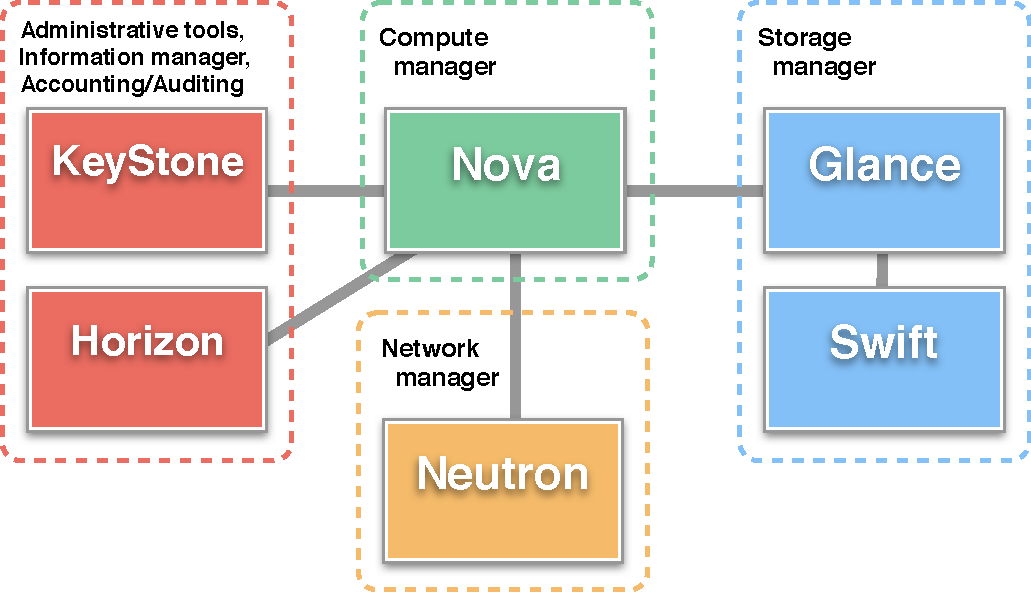
\includegraphics[width=6cm]{figures/OpenStack_architecture.pdf}
\vspace*{-.3cm}
        \caption{Services composing OpenStack.}
        \label{fig:openstack}
\vspace*{-.3cm}
\end{figure}


OpenStack relies on two kinds of nodes: controller nodes and compute nodes. The
formers are in charge of managing and distributing work to the latters that
provide computing/storage resources to end-users. In other words, controller
nodes correspond to the different services introduced in the previous
section while compute nodes are dedicated to the hosting of VMs.

The software architecure of services composing OpenStack is based on the
``shared nothing" principles: each controller node (\ie each service) is 
connected to the other controllers via two different ways:

\begin{itemize}
   \setlength{\itemsep}{0pt}
  \setlength{\parskip}{0pt}
   \setlength{\parsep}{0pt}
\item \textbf{A messaging queue}, implementing the AMQP protocal that enables
the collaboration between sub-services of a controller.
\item \textbf{A relational database} (DB) that stores inner states of a controller.
\end{itemize}

Finally, the controllers interact with each others through REST APIs or directly
by accessing the inner-states (i.e. logical objects used by OpenStack for its
functionning) stored in several database backends (mainly MySQL).
%\AL[JP]{Is it correct ? How the controllers interaact/collabore ?}

Indeed, the process of revising OpenStack, towards a more decentralized and an
advanced distributed functionning, can be carried out in two ways: the
decentralization of the messaging queue and the use of an alternative to
relational databases.

\subsection{Decentralizing the AMPQ Messaging Queue}

OpenStack relies on the RabbitMQ messaging service, which is articulated around
the concept of centralized broker. RabbitMQ provide by default a cluster mode, 
which can be configured to work in a high available mode: several machines,
each hosting a RabbitMQ instance, work together in an Active/Active functionning
where each queues is mirrored on all nodes. This mode is recommended by the
documentation for setting up a multi-controller nodes OpenStack infrastructure.
While it has the advantage of being simple, it has the drawback of being very
sensible to network latency, and thus is not relevant for multi-site
configurations.

According to RabbitMQ documentation, it is possible to use different modes such
cluster federation of shovels. This represents a first lead to decentralize the
AMQP messaging queue used by OpenStack services. Alternatively, there are few
implementations of P2P messaging service such as ActiveMQ~\cite{activemq:2011}
or ZeroMQ~\cite{zeromq:2013} that would be adapted to the LUC requirements.

% \section{Towards a fully distributed OpenStack deployment}
%
% The discovery initiative targets the delivery of an utility computing platform
% that will be working on top of existing network backbone facilities. Starting
% the development of such a platform from zero would require a titanic effort: in
% order to spare a giant development time, the Discovery initiative proposes to
% leverage the OpenStack project: this will serve as the foundation of the
% LUC-OS.
%
% In order to structure the LUC-OS on a fully distributed peer to peer
% functionning, OpenStack would be required to be fault tolerant and to be able to
% fit on a multi-site configuration. In the current situation, it requires some
% adaptations: in this section we propose some modifications that
% have been introduced in the Nova controller, to meet the two
% aforementioned criterions.
%
% \subsection{Replacing the relational backend by a Key/value store}
%


\subsection{Enabling the support of NoSQL databases in Nova}

\begin{figure*}
  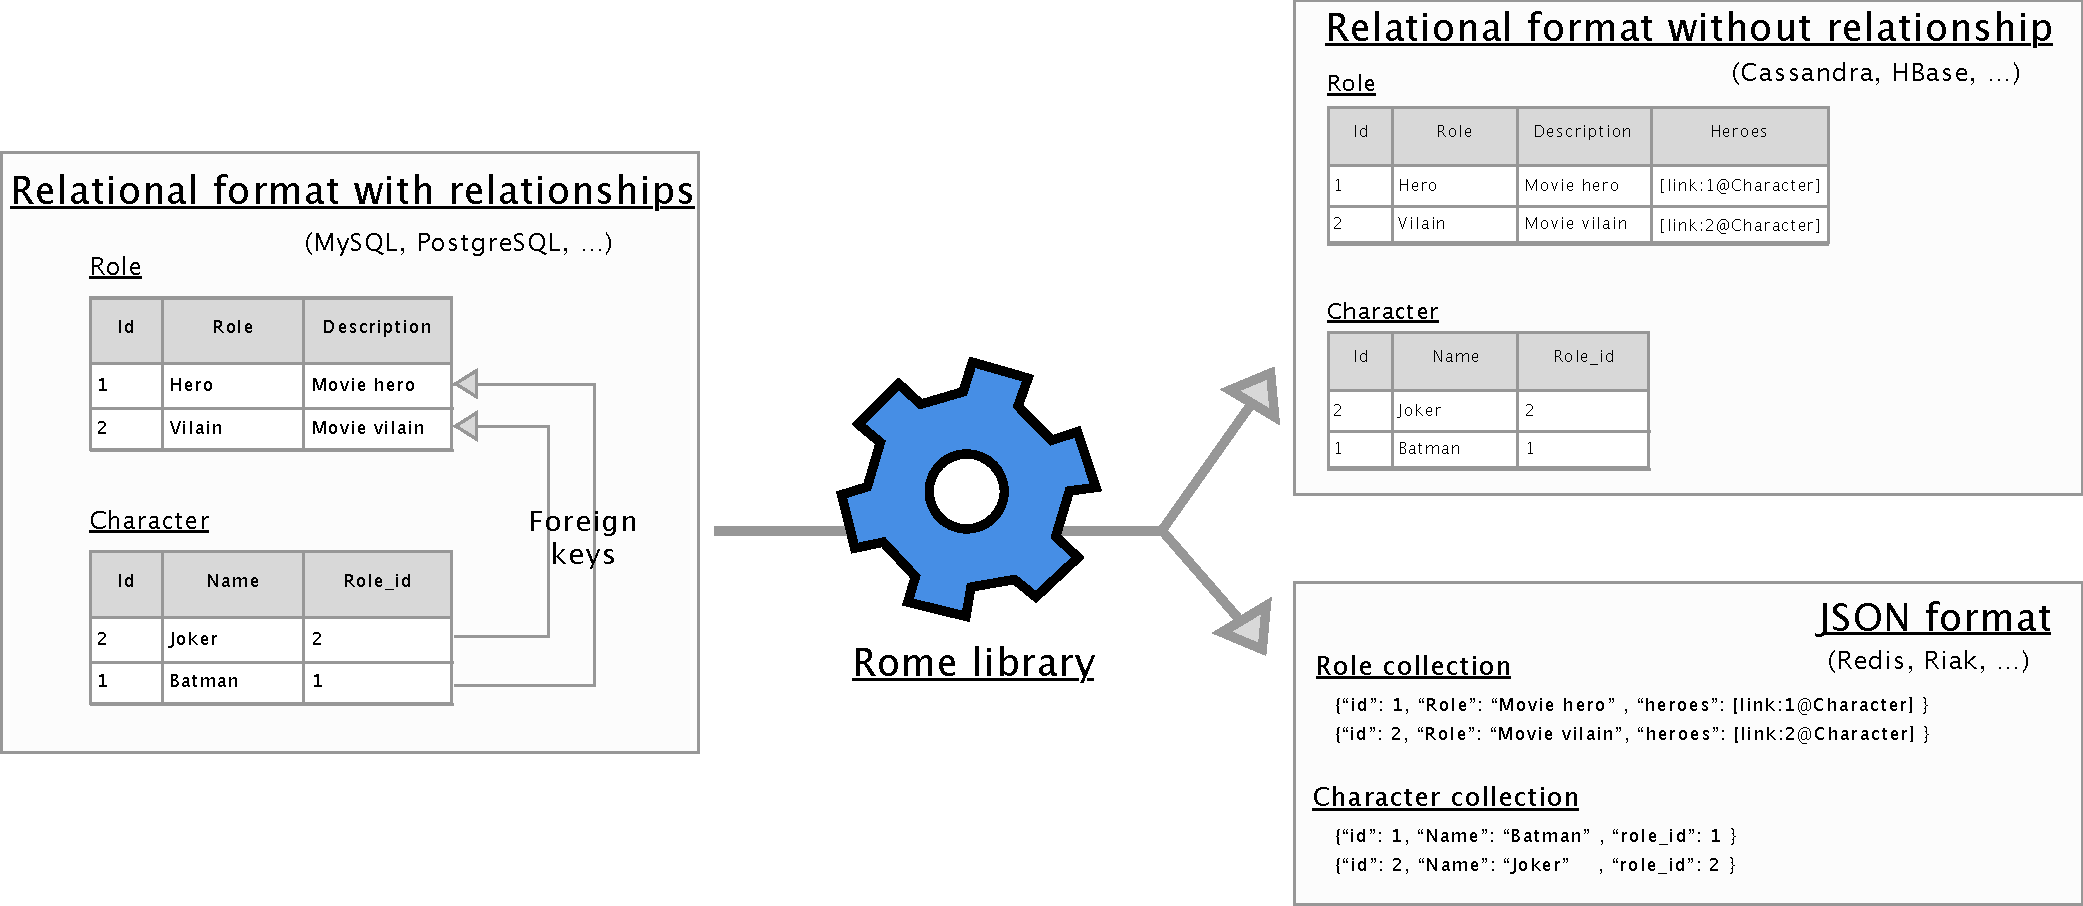
\includegraphics[width=.99\textwidth]{figures/rome_models.pdf}
  \caption{Rome is a library that enables to work with NoSQL databases with an object oriented interface.}
  \label{fig:rome_format}
\end{figure*}


From today's perspective, most of the OpenStack deployments are involving few
nodes, thus not requiring more than a single controller node. For larger
deployments, involving several controller nodes, there are several possibility
considering the architecture of the database: a first possibility would be to
use a single database server shared between all the controller nodes, which has
the advantage of being a simple solution at the cost of introducing a single
point of failure (SPOF) in case the server crashes. The second possibility is to
follow recommendations proposed by OpenStack documentation and  to deploy on
each controller a DB which will be synchronized with the DBs of other servers
with instances with a dedicated mechanism~\cite{kemme:vldb2010}. By such a mean,
when a controller processes a request and performs some actions on one site,
changes in the inner-state are also propagated to all the other locations. From
a certain point of view, it gives the illusion that there is only one DB for
each service. Although the technique described has been used in different proof-
of- concepts, current DB synchronization mechanisms are not scalable enough to
cope with a LUC infrastructure deployed on large number of geographical sites.

Another approach would be to replace the DBs used in OpenStack by a more
suitable storage backend that would provide a better scalability, like NoSQL
databases. Distributed Hash Tables (DHTs) and more recently key/value systems
built on top of the DHT concept such as \emph{Dynamo}~\cite{decandia:dynamo}
have demonstrated their efficiency in terms of scalability and fault tolerance
properties. On the other hand, there exists NoSQL databases that provide
interfaces clother to relational databases, as Cassandra which is fully
distributed while supporting queries in a subset of the SQL language (CQL).


\subsubsection{Rome library}

OpenStack doesn't manipulate directly data stored on the relational database,
instead it uses \textit{SQLAlchemy} which serves as an Object-Relationnal
mapping tool by making the link between the relational format used by database
and the object  format used by programs. Thus OpenStack services manipulates
inner-states stored in the database with an object oriented vision.

In light of this, we have developed a python library called \textit{``Rome"}
which targets at enabling python programs to manipulate data stored in NoSQL
databases with the same programmatic interfaces provided by \textit{SQLAlchemy}.
As there exists several types of NoSQL databases (Key/Values stores like Redis,
column oriented databases like Cassandra, ...), Rome supports several types of
databases, enabling to manipulate them with the same programmatic interfaces.

\textit{Rome} provides the support of relationships in NoSQL databases: 
relationships between tables are widely used in relational databases thanks to
the concept of foreign keys, and most of the NoSQL databases do not implement
this. \textit{Rome} support the definition of relationships between model
classes, and thus enables to propagate modifcation on an object to its linked
objects.

Moreover, \textit{Rome} implements the \textit{join} technic that enables to
combine rows of several tables, in the same manner as SQLAlchemy do. While
SQLAlchemy leverage the ``JOIN" operator in SQL language and thus delagate the
work to the database server, \textit{Rome} cannot do the same as most of the
NoSQL databases (REDIS, Cassandra) do not implement the ``JOIN" operation: this
operation is executed by ``ROME", on the client-side, thus maintaining the
compatibility with \textit{SQLAlchemy}.

Finally, \textit{Rome} enables the support of transactions as defined by
\textit{SQLAlchemy}: while \textit{SQLAlchemy} rely on transactional mechanisms
provided by database server, \textit{Rome} simulates this operation thanks to
a distributed lock implemented with \textit{REDIS} that enables to lock model
objects and use timeout measurement to detect deadlock situations.

\subsubsection{Combining Nova with REDIS}

Leveraging the \textit{Rome} library, we have revisited the Nova service which
is in charge of managing VMs manager deployed in an OpenStack infrastructure, in
order to to replace the current MySQL DB system by \textit{REDIS}
~\cite{han:2011}, a \textit{key/value store}. Technically speaking, we modified
the Nova database driver. Indeed, the  Nova software architecture has been
organised in a way which ensures that each of its sub-services does not directly
manipulate the database: they have an indirect access through a service called
``nova- conductor" which in turn works with an implementation of the
\textbf{"nova.db.api"} programming interface. Developers of Nova provide an
implementation of this interface that is using \textit{SQLAlchemy} to manipulate
a relational database. We developed a second implementation of this interface
that replaces every call to the \textit{SQLAlchemy} by a call to a custom
key/value store driver.  This enables  Nova's services to work with REDIS by
only changing the database driver, limiting the level of intrusiveness in the
original source code. Thanks to this modification, it is possible to instanciate
a distributed cloud and operate it through a single instance of OpenStack
composed of several Nova controllers deployed on distinct sites.
Figure~\ref{fig:newnova} depictes such a deployment.

Each controller executes a REDIS instance that is configured to work in a
clustering way with other instances. One or several controllers can be deployed
on each site according to the expected demand in terms of end-users. Finally, a
controller can be deployed either on a dedicated node or be mutalized with a
compute one as illustrated for Site 3. We higlight that any controller can
provision VMs by orchestrating services on the whole infrastructure and not only
on the site where it is deployed. Such a behavior is possible thanks to the AMQP
bus and the key/value store that go through all controllers.

Finally, it is noteworthy that key/value stores that focus on high-availability
and partition tolerance criteria like Cassandra~\cite{lakshman:2010} would be
more appropriate than REDIS for a production deployment. We chose REDIS for its
usage simplicity.

\begin{figure}[htbp]
        \centering
\vspace*{-.4cm}        \hspace*{-.2cm}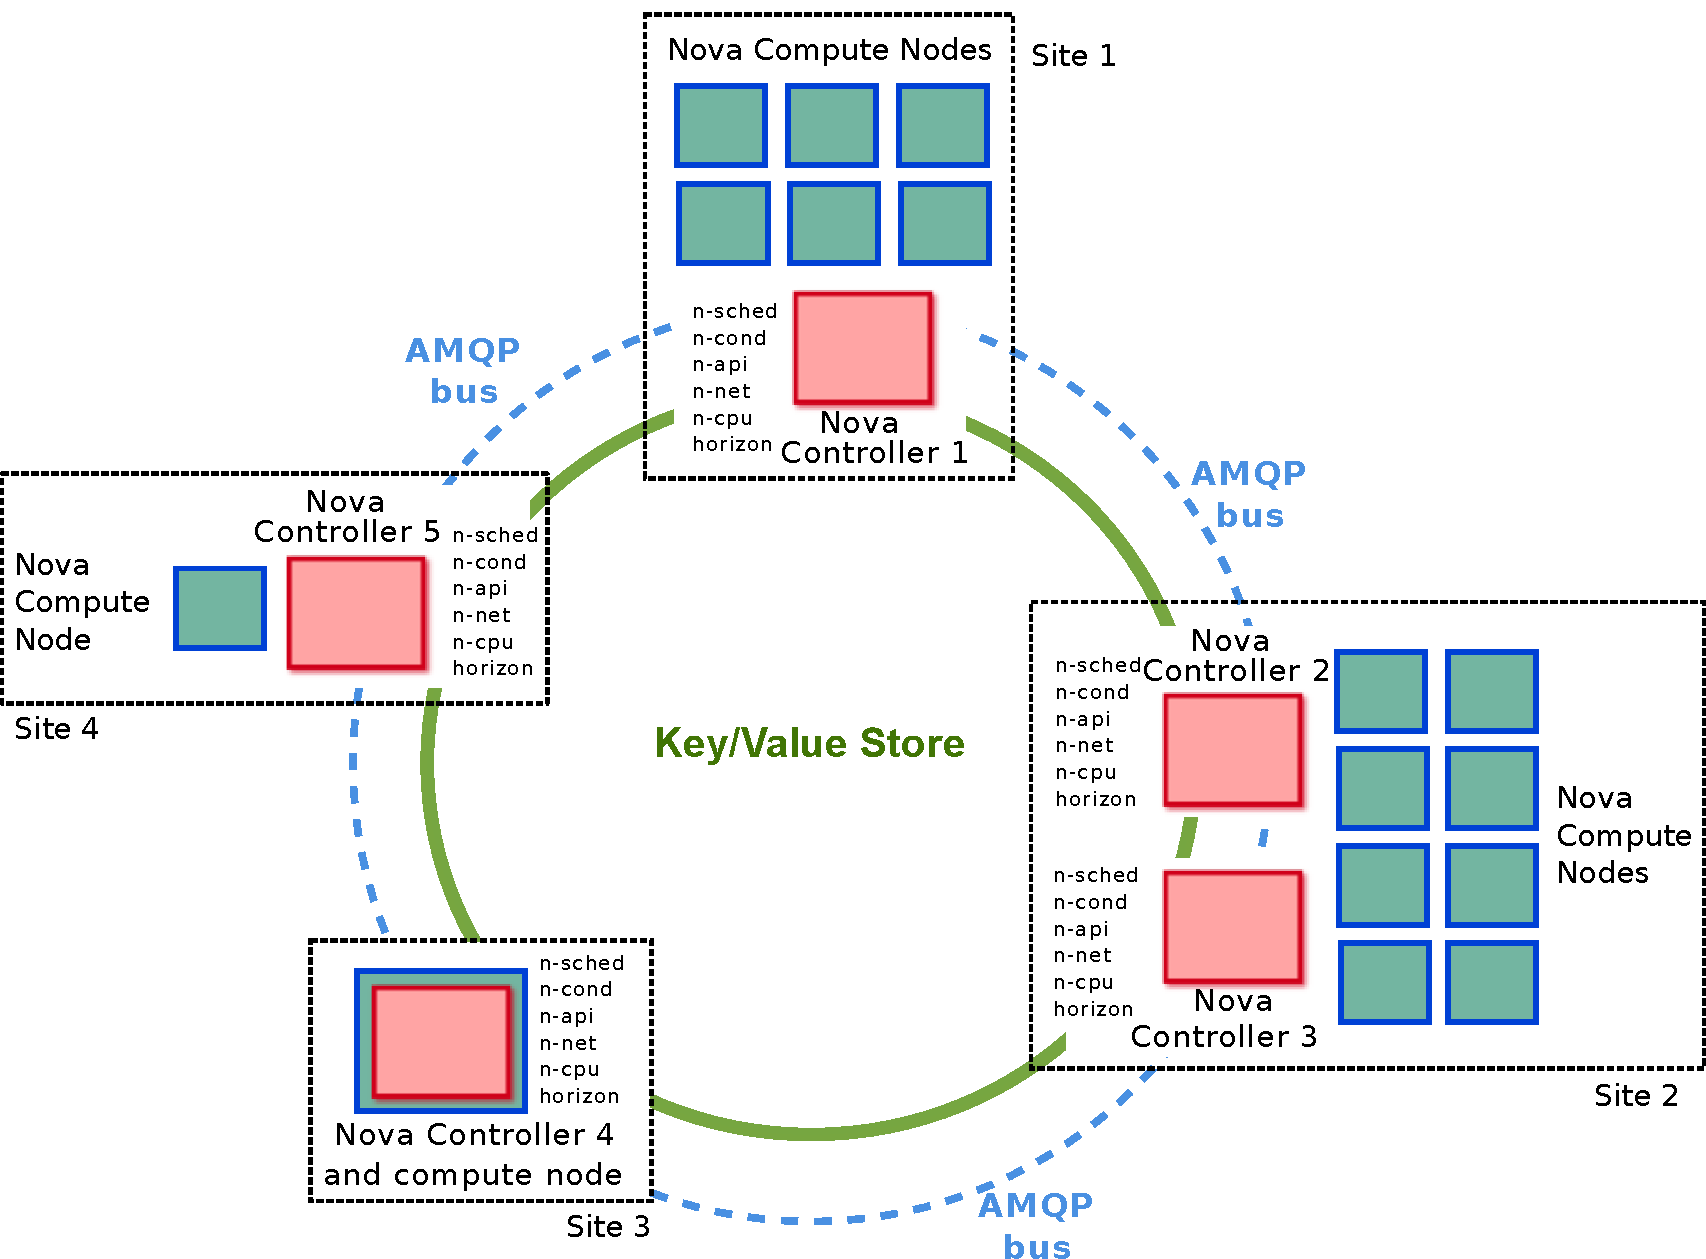
\includegraphics[width=.51\textwidth]{figures/OpenStack_distributed.pdf}
        \caption{Nova controllers are connected through a shared key/value backend
        and the AMQP bus.}
      \label{fig:newnova}
\vspace*{-.3cm}
\end{figure}

Our prototype is under evaluation. However, preliminary experiments  have been
performed throughout 4 sites of Grid'5000  including 12 compute nodes  and 4
controllers overall. While this infrastructure was rather small in comparison to
our target, it aimed at validating the interconnection of several controllers
WANwide and the correct behaviour of  OpenStack using our noSQL backend. Our
prototype suceeded to provision 500 VMs in 300 seconds (each controller creating
125 VMs in parallel). A second experiment validated the provisionning of 2000
VMs in less than 30 min.  We are currently performing comparisons between
OpenStack using the historical MYSQL backend \textit{v.s.,} using a key/value
store backend. Our goal is to validate that manipulating internal states of
Openstack through a noSQL deliver performances in the same order of the MySQL
ones.
